L'odierna rete elettrica è stata progettata come un sistema centralizzato, in cui l'energia elettrica fluisce attraverso linee unidirezionali di trasmissione e distribuzione dai generatori fino ai clienti finali. La logica applicativa è concentrata in zona centrale e solo parzialmente nelle \emph{substations}, mentre le componenti restanti sono totalmente passive. Le Smart Grid forniscono una più elevata ed ampia intelligenza distribuita incorporata nei dispositivi locali, comunicazione e scambio bidirezionale di informazioni ed elettricità.

\section{Smart Grid Framework}
Le Smart Grid richiedono sia una complessa infrastruttura di comunicazione, che sofisticate tecnologie di comunicazione e computazione. Entrambe consentono la conservazione di parte dell'energia prodotta e l'introduzione di nuovi metodi di gestione della domanda energetica, per adottare politiche di bilanciamento del carico, controllare instabilità energetiche causate dalla natura delle risorse rinnovabili e prevenire la diffusione di fallimenti in cascata nella rete. 
\newline 
La figura \ref{fig:1} riassume le principali tematiche relative alle Smart Grid:
\begin{itemize}
	\item energy infrastructure rappresenta la base fisica ed organizzativa necessaria per la generazione, trasmissione e distribuzione dell'energia;
	\item communication infrastructure è responsabile del trasferimento di informazioni critiche attraverso la rete;
	\item information technology fornisce modelli, analisi, visualizzazioni web e transazioni commerciali;
	\item potential applications offre tecniche di generazione, gestione, automatizzazione e rilevamento per l'intero sistema.
\end{itemize} 

\begin{figure}[h] \centering{
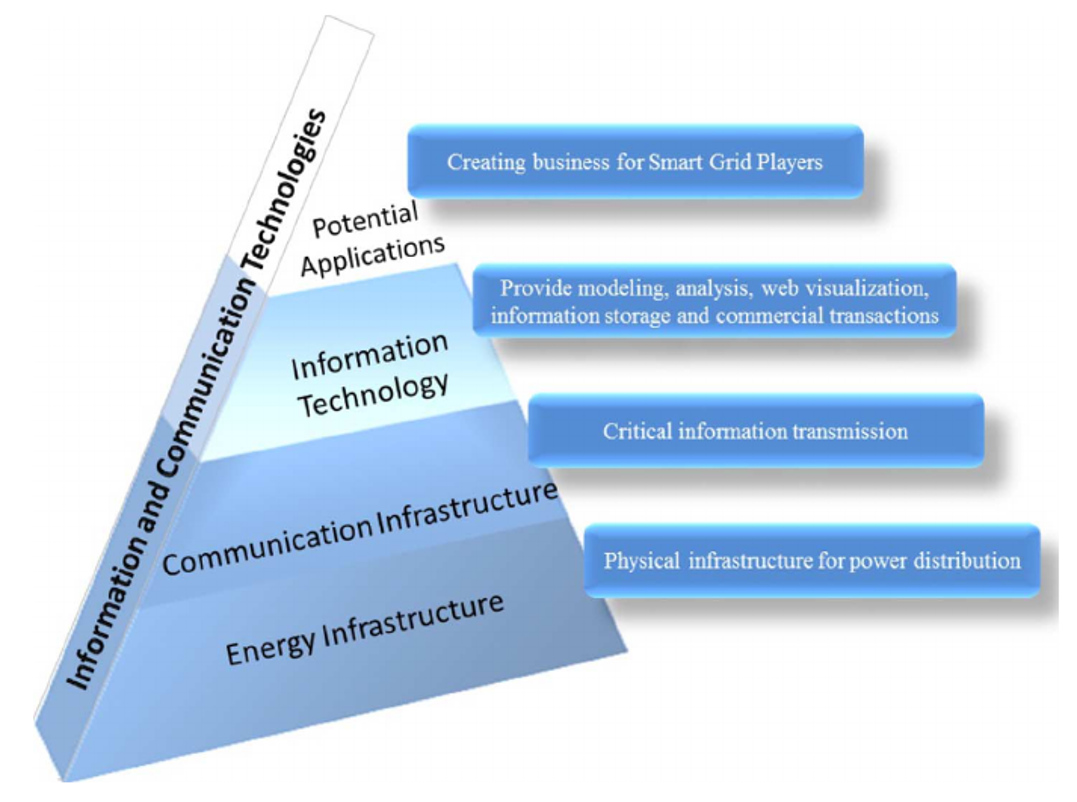
\includegraphics[scale=0.3, natwidth=1003,natheight=490]{imgs/ict.png}}
\caption{Smart Grid framework}\label{fig:1}
\end{figure}

La communication infrastructure svolge un ruolo cruciale, ossia collegare tutte le componenti della rete collezionando informazioni sulle loro condizioni, per scopi di controllo, monitoraggio e manutenzione. Eventuali problemi legati all'energy instrastructure possono essere evitati se corrette operazioni vengono prese con l'aiuto della communication infrastructure. 
\newline 
Differenti tecnologie di comunicazione posso essere usate per diversi scopi e requisiti in base all'applicazione. L'information technology fornisce una piattaforma comune di scambio di informazioni proveniente da differenti attività legate alla Smart Grid, che permette l'integrazione di informazioni da diversi livelli, dando sostegno alla raccolta di diverse informazioni, all'analisi e ad applicazioni avanzate.
\newline
Le tecniche dell'applications layer generalmente mirano a ridurre il consumo energetico dei clienti, cambiando i loro comportamenti di consumo, dotandoli di strumenti di monitoraggio.    

\newpage
La figura \ref{fig:2} mostra le componenti della Smart Grid, illustrate dall'energy infrastructure al potentional applications.

\begin{figure}[h] \centering{
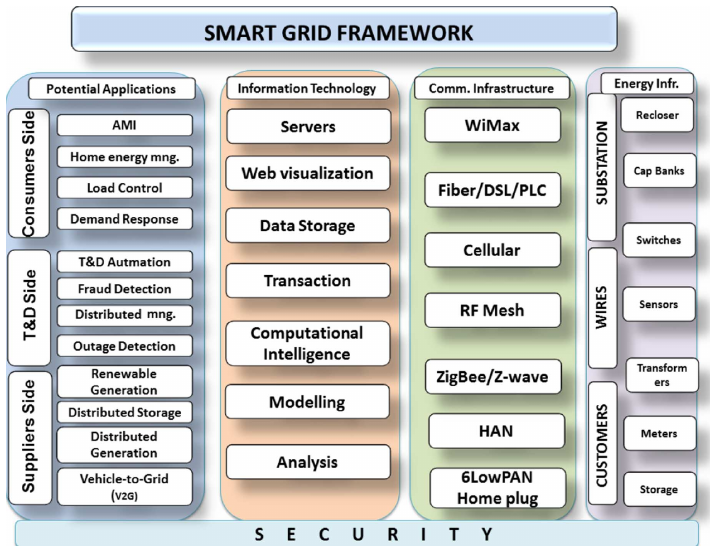
\includegraphics[scale=0.7, natwidth=1003,natheight=490]{imgs/sgframework.png}}
\caption{Smart Grid framework}\label{fig:1}
\end{figure}

% http://ieeexplore.ieee.org/stamp/stamp.jsp?tp=&arnumber=6298960 